\documentclass{article}
\usepackage{graphicx}
\usepackage[margin=1.5cm]{geometry}
\usepackage{amsmath}
\usepackage{fancyvrb}
\usepackage{url}

\begin{document}

\title{Synopsis - Week 7 Integrated Project: fixed IC gates and counters, gates and counters in programmable logic}
\author{Prof. Jordan C. Hanson}

\maketitle

\section{Finite Impulse Response (FIR) Filter}

\noindent
A finite impulse response (FIR) filter takes digitized data as the input, and returns modified data of the same shape as the output.  Let $n$ represent the number of samples of digitized data.  Let $x[n]$ represent the vector of digitized input data, and $y[n]$ represent the digitized output data.  Let $z^{-1}$ represent an operation that selects the prior sample, or the $n-1$ sample relative to sample $n$.  Let the coefficients $b_n$ multiply the samples $x[n]$ as they pass through an amplifier.  Finally, let $\Sigma$ represent an adder that sums to inputs and produces one output.  A generalized circuit diagram for the FIR filter is shown in Fig. \ref{fig:fir}, and the formula relating the input to the output is given in Eq. \ref{eq:fir}.

\begin{figure}[ht]
\centering
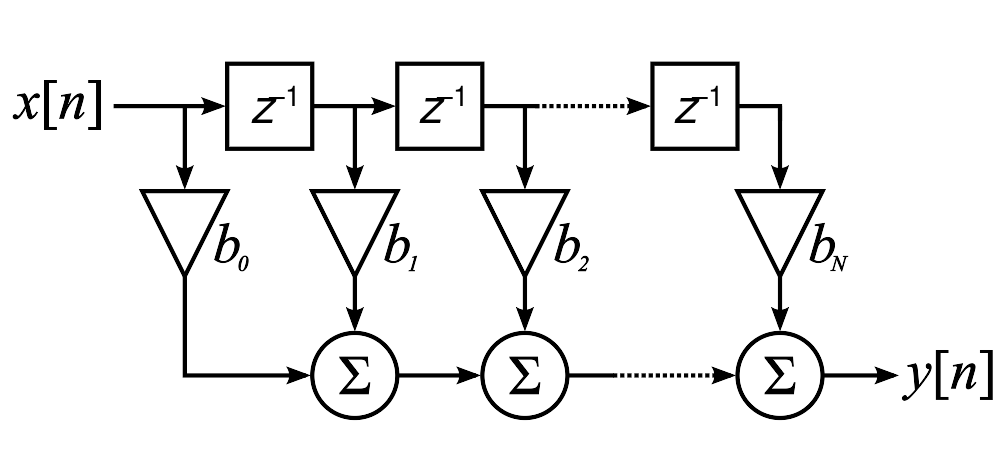
\includegraphics[width=0.33\textwidth]{figures/FIR_Filter.png}
\caption{\label{fig:fir} A generalized circuit diagram for the FIR filter.}
\end{figure}

\begin{equation}
y[n] = \sum_{i=0}^N b_i x[n-i]
\end{equation}

In this lab, we are going to create a PYNQ overlay that will implement Eq. \ref{fig:fir} in the SoC PL layer.

\section{Comparing fixed IC gates and counters to programmable logic}

\begin{enumerate}
\item Things
\end{enumerate}

\end{document}
